GuppyLM is a deliberately tiny, open-source and character-driven language model, themed as
a fish. It was built for teaching, being a complete and readable reference implementation
of a small instruction-tuned transformer, and it is a good mechanism testbed precisely
because it is small enough to be fully controllable and inspectable while still being a
real instruction-tuned transformer. Its architecture and training data are summarised in
Table~\ref{tab:guppylm_properties}.

\begin{table}[htbp]
\centering
\caption{GuppyLM architecture and training data.}
\label{tab:guppylm_properties}
\begin{tabular}{l l}
\toprule
\textbf{Property} & \textbf{Value} \\
\midrule
Parameters &  $\approx 8.73$M \\
Transformer blocks & 6 \\
Hidden dimension $k$ & 384 \\
Vocabulary capacity & 4096 \\
Training data & \href{https://huggingface.co/datasets/arman-bd/guppylm-60k-generic}{$\approx 60$k rows over 60 categories} \\
\bottomrule
\end{tabular}
\end{table}

Each block outputs a residual-stream tensor of shape $[B, T, 384]$, which matches the
method of Beaglehole et al. for reading from and writing to the model. The model is
trained on 60 templated conversational categories, such as food, weather, greetings and
moods, and those categories are the only concepts GuppyLM can plausibly be expected to
represent, given that they are the whole of its training distribution, so we restrict this
work to them. Note that whether the model also carries structure outside these categories
is not something we tested, and it is not something a probe restricted to these labels
could see.

One convenient consequence of GuppyLM's small scale is that its per-block activation norms
are small and can simply be measured. The median $\|a_\ell\|_2$ over the cached training
activations runs $11.9,\ 22.8,\ 27.6,\ 30.7,\ 30.9,\ 29.7$ from block 0 to block 5, a
roughly $2.6$-fold rise that peaks at block 4, as shown in
Figure~\ref{fig:activation_norms}. Consequently a fixed absolute perturbation is a nudge
at block 5 and a wrecking ball at block 0, which is exactly why the absolute steering
coefficients of Beaglehole et al. cannot be copied over.

\begin{figure}[htbp]
    \centering
    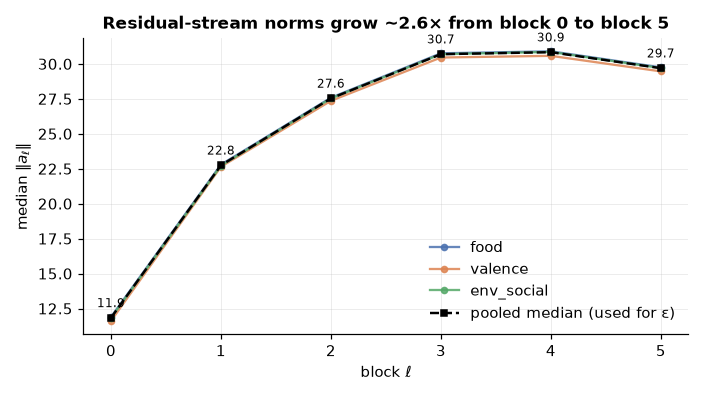
\includegraphics[width=0.75\textwidth]{imgs/01_activation_norms.png}
    \caption{The three concepts agree almost exactly, and the median (dashed) is a safe scale to normalise by.}
    \label{fig:activation_norms}
\end{figure}

It is possible to see in the figure that the three concepts agree almost exactly on the
per-block norm profile, which means the median is a safe common scale to normalise by, and
it is that median which defines the relative coefficient $r$ used throughout the steering
experiments below.
